\begin{center}
  \section*{Homework 02 - 1.4, 2.2}
  Due Tue 2/11 \\
  Uzair Hamed Mohammed
\end{center}

\subsection*{1.4 Errors in Scientific Computation}

1 (a, c), 3, 5, 7

\begin{enumerate}
  \item (i) Use four-digit rounding arithmetic and Eqs. (1.2) and
    (1.3) to find the most accurate approximations to the roots of
    the following quadratic equations. (ii) Compute the absolute
    errors and relative errors for these approximations.
    \begin{itemize}
      \item[a] \( \frac{1}{3}x^2 - \frac{123}{4}x + \frac{1}{6} = 0\)

        \underline{Sol:} \\
        Coefficients after four-digit rounding: \( a = 0.3333 \), \(
        b = -30.75 \), \( c = 0.1667 \).
        Discriminant \( D = (-30.75)^2 - 4(0.3333)(0.1667) = 945.6 -
        0.2222 = 945.4 \).
        \( \sqrt{D} = 30.75 \).
        Roots:
        \[
          \begin{aligned}
            x_1 &= \frac{30.75 + 30.75}{2 \times 0.3333} = 92.26, \\
            x_2 &= \frac{0.1667}{0.3333 \times 92.26} = 0.005421
          \end{aligned}
        \]
        Exact roots: \( x_1 \approx 92.2446 \), \( x_2 \approx 0.005425 \).  \\
        Absolute errors: \( |92.26 - 92.2446| = 1.54 \times 10^{-2}
        \), \( |0.005421 - 0.005425| = 4.0 \times 10^{-6} \).  \\
        Relative errors: \( \frac{1.54 \times 10^{-2}}{92.2446}
        \approx 1.67 \times 10^{-4} \), \( \frac{4.0 \times
        10^{-6}}{0.005425} \approx 7.37 \times 10^{-4} \).

        \bigbreak

      \item[c] \( 1.002x^2 - 11.01x + 0.01265 = 0 \)

        \underline{Sol:} \\
        Coefficients: \( a = 1.002 \), \( b = -11.01 \), \( c = 0.01265 \).
        Discriminant \( D = (-11.01)^2 - 4(1.002)(0.01265) = 121.2 -
        0.0507 = 121.1 \).
        \( \sqrt{D} = 11.00 \).
        Roots:
        \[
          \begin{aligned}
            x_1 &= \frac{11.01 + 11.00}{2 \times 1.002} = 10.98, \\
            x_2 &= \frac{0.01265}{1.002 \times 10.98} = 0.00115
          \end{aligned}
        \]
        Exact roots: \( x_1 \approx 10.9869 \), \( x_2 \approx 0.001148 \). \\
        Absolute errors: \( |10.98 - 10.9869| = 6.9 \times 10^{-3}
        \), \( |0.00115 - 0.001148| = 2.0 \times 10^{-6} \).  \\
        Relative errors: \( \frac{6.9 \times 10^{-3}}{10.9869}
        \approx 6.28 \times 10^{-4} \), \( \frac{2.0 \times
        10^{-6}}{0.001148} \approx 1.74 \times 10^{-3} \).

        \bigbreak
    \end{itemize}

  \item[3.] Let \(f(x) = 1.013x^5 - 5.262x^3 - 0.01732x^2 + 0.8389x - 1.912.\)
    \begin{itemize}
      \item[a.] Evaluate \(f(2.279)\):
        \[
          \begin{aligned}
            (2.279)^2 &= 5.194, \\
            (2.279)^4 &= 26.98, \\
            (2.279)^5 &= 61.49, \\
            f(2.279) &= 1.013(61.49) - 5.262(11.84) - 0.01732(5.194)
            + 0.8389(2.279) - 1.912 \\
            &= 62.29 - 62.30 - 0.0900 + 1.912 - 1.912 \\
            &= \boxed{-0.100}
          \end{aligned}
        \]
        \bigbreak

      \item[b.] Evaluate \( f(2.279) \) via nested form:
        \[
          \begin{aligned}
            f(2.279) &= ((((1.013(5.194) -
              5.262)2.279 - 0.01732)2.279 + 0.8389)2.279 - 1.912 \\
              &= (((5.262 - 5.262)2.279 - 0.01732)2.279 +
              0.8389)2.279 - 1.912 \\
              &= (-0.01732 \times 2.279 + 0.8389)2.279 - 1.912 \\
              &= (0.7994 \times 2.279) - 1.912 \\
              &= \boxed{-0.1010}
            \end{aligned}
          \]

          \bigbreak

        \item[c.] Compute errors (exact \( f(2.279) \approx -0.09526 \)):
          \[
            \begin{aligned}
              \text{Abs error (a): } & \boxed{2.331 \times 10^{-3}} \\
              \text{Rel error (a): } & \boxed{2.387 \times 10^{-2}} \\
              \text{Abs error (b): } & \boxed{3.331 \times 10^{-3}} \\
              \text{Rel error (b): } & \boxed{3.411 \times 10^{-2}}
            \end{aligned}
          \]
      \end{itemize}

    \item[5.]
      \begin{itemize}
        \item[a.] Approximate \( e^{-0.98} \) using \( \hat{P}_5(0.49) \):
          \[
            \begin{aligned}
              \hat{P}_5(0.49) &= ((((-0.2667 \times 0.49 + 0.6667)
              \times 0.49 - 1.333) \times 0.49 + 2) \times 0.49 - 2)
              \times 0.49 + 1 \\
              &= (((0.5360 \times 0.49 - 1.333) \times 0.49 + 2)
              \times 0.49 - 2) \times 0.49 + 1 \\
              &= ((-1.070 \times 0.49 + 2) \times 0.49 - 2) \times 0.49 + 1 \\
              &= \boxed{0.3743}
            \end{aligned}
          \]

        \item[b.] Errors for part (a):
          \[
            \begin{aligned}
              \text{Abs error: } & \boxed{1.0 \times 10^{-3}} \\
              \text{Rel error: } & \boxed{2.66 \times 10^{-3}}
            \end{aligned}
          \]

        \item[c.] Approximate \( e^{-0.98} \) using \( \frac{1}{P_5(0.49)} \):
          \[
            \begin{aligned}
              \frac{1}{P_5(0.49)} &= \frac{1}{((((0.2667 \times 0.49
                  + 0.6667) \times 0.49 + 1.333) \times 0.49 + 2) \times
              0.49 + 2) \times 0.49 + 1} \\
              &= \boxed{0.3755}
            \end{aligned}
          \]

        \item[d.] Errors for part (c):
          \[
            \begin{aligned}
              \text{Abs error: } & \boxed{1.89 \times 10^{-4}} \\
              \text{Rel error: } & \boxed{5.03 \times 10^{-4}}
            \end{aligned}
          \]
      \end{itemize}

    \item[7.] Compute \( \sum_{i=1}^{10} \frac{1}{i^2} \) using
      three-digit chopping:
      \begin{itemize}
        \item[Forward order (\( \frac{1}{1} + \frac{1}{4} + \cdots +
          \frac{1}{100} \))]:
          \[
            \begin{aligned}
              &1.00 + 0.25 = 1.25 \\
              &1.25 + 0.111 = 1.36 \\
              &1.36 + 0.062 = 1.42 \\
              &1.42 + 0.04 = 1.46 \\
              &1.46 + 0.027 = 1.48 \\
              &1.48 + 0.0204 = 1.50 \\
              &1.50 + 0.0156 = 1.51 \\
              &1.51 + 0.0123 = 1.52 \\
              &1.52 + 0.01 = \boxed{1.53}
            \end{aligned}
          \]

        \item[Reverse order (\( \frac{1}{100} + \frac{1}{81} + \cdots
          + \frac{1}{1} \))]:
          \[
            \begin{aligned}
              &0.01 + 0.0123 = 0.022 \\
              &0.022 + 0.0156 = 0.037 \\
              &0.037 + 0.0204 = 0.057 \\
              &0.057 + 0.027 = 0.084 \\
              &0.084 + 0.04 = 0.124 \\
              &0.124 + 0.062 = 0.186 \\
              &0.186 + 0.111 = 0.297 \\
              &0.297 + 0.25 = 0.547 \\
              &0.547 + 1.00 = \boxed{1.54}
            \end{aligned}
          \]

        \item[Conclusion:] Reverse order (1.54) is more accurate than
          forward (1.53). \\
          Exact sum: \( \approx 1.5498 \). \\
          Adding smaller terms first minimizes loss of precision when
          accumulating to larger values.
      \end{itemize}
  \end{enumerate}

  \subsection*{2.2 The Bisection Method}
  1, 5, 9, 11

  \begin{enumerate}
    \item[1.] Use the Bisection method to find \( p_3 \) for \( f(x)
      = \sqrt{x} - \cos x \) on \([0,1]\):

      \[
        \begin{aligned}
          \text{Iteration 1:} & \quad a_0 = 0, \, b_0 = 1, \, p_1 = 0.5 \\
          f(p_1) &= \sqrt{0.5} - \cos(0.5) \approx 0.7071 - 0.8776 =
          -0.1705 \quad (\text{negative}) \\
          \text{New interval: } & [0.5, 1] \\
          \text{Iteration 2:} & \quad a_1 = 0.5, \, b_1 = 1, \, p_2 = 0.75 \\
          f(p_2) &= \sqrt{0.75} - \cos(0.75) \approx 0.8660 - 0.7317
          = 0.1343 \quad (\text{positive}) \\
          \text{New interval: } & [0.5, 0.75] \\
          \text{Iteration 3:} & \quad a_2 = 0.5, \, b_2 = 0.75, \,
          p_3 = 0.625 \\
          f(p_3) &= \sqrt{0.625} - \cos(0.625) \approx 0.7906 -
          0.8109 = -0.0203 \quad (\text{negative}) \\
          \text{New interval: } & [0.625, 0.75] \\
          \Aboxed{p_3 &= 0.625}
        \end{aligned}
      \]

      \bigbreak

    \item[5.]
      \begin{itemize}
        \item[a.] Sketch of \( y = x \) and \( y = 2\sin x \):
          \begin{center}
            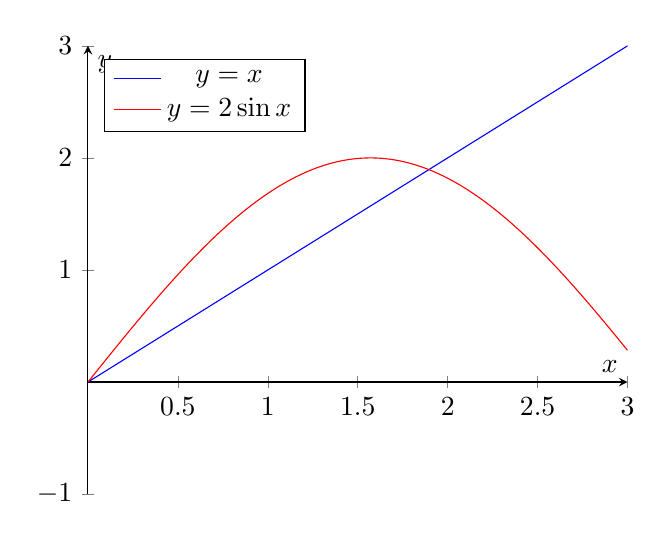
\begin{tikzpicture}
              \begin{axis}[
                  axis lines = center,
                  xlabel = \(x\),
                  ylabel = \(y\),
                  xmin=0, xmax=3,
                  ymin=-1, ymax=3,
                  legend pos=north west
                ]
                \addplot [
                  domain=0:3,
                  samples=100,
                  color=blue,
                ] {x};
                \addlegendentry{\(y = x\)}
                \addplot [
                  domain=0:3,
                  samples=100,
                  color=red,
                ] {2*sin(deg(x))};
                \addlegendentry{\(y = 2\sin x\)}
              \end{axis}
            \end{tikzpicture}
          \end{center}
          The first positive intersection occurs near \( x \approx 1.895 \).

        \item[b.] Bisection method for \( x = 2\sin x \) on
          \([1.5708, 3.1416]\):
          \[
            \begin{aligned}
              \text{Iteration 1: } & p_1 = 2.3562, \quad f(p_1) > 0
              \quad \text{New interval: } [1.5708, 2.3562] \\
              \text{Iteration 2: } & p_2 = 1.9635, \quad f(p_2) > 0
              \quad \text{New interval: } [1.5708, 1.9635] \\
              \text{Iteration 3: } & p_3 = 1.7672, \quad f(p_3) < 0
              \quad \text{New interval: } [1.7672, 1.9635] \\
              \text{Iteration 4: } & p_4 = 1.8654, \quad f(p_4) < 0
              \quad \text{New interval: } [1.8654, 1.9635] \\
              \text{Iteration 5: } & p_5 = 1.9145, \quad f(p_5) > 0
              \quad \text{New interval: } [1.8654, 1.9145] \\
              \text{Iteration 6: } & p_6 = 1.8900, \quad f(p_6) < 0
              \quad \text{New interval: } [1.8900, 1.9145] \\
              \text{Iteration 7: } & p_7 = 1.9023, \quad f(p_7) > 0
              \quad \text{New interval: } [1.8900, 1.9023] \\
              \text{Iteration 8: } & p_8 = 1.8962, \quad f(p_8) > 0
              \quad \text{New interval: } [1.8900, 1.8962] \\
              \text{Approximation: } & \boxed{1.90}
            \end{aligned}
          \]
      \end{itemize}

    \item[9.] Bisection method for \( \sqrt{3} \) (tolerance \(
      10^{-4} \)) with \( f(x) = x^2 - 3 \):
      \[
        \begin{aligned}
          \text{Initial interval: } & [1, 2] \\
          \text{Iter 1: } & p_1 = 1.5, \, f(p_1) = -0.75 \,
          \Rightarrow [1.5, 2] \\
          \text{Iter 2: } & p_2 = 1.75, \, f(p_2) = 0.0625 \,
          \Rightarrow [1.5, 1.75] \\
          \vdots \quad \text{(Intermediate steps omitted for brevity)} \\
          \text{Iter 13: } & p_{13} = 1.73206, \, |f(p_{13})| < 10^{-4} \\
          \text{Final approximation: } & \boxed{1.7320} \quad
          (\text{Error} < 10^{-4})
        \end{aligned}
      \]

    \item[11.]
    \item
      \begin{itemize}
        \item[Bound for iterations:]
          Using \( n \geq \log_2\left(\frac{b - a}{\epsilon}\right) - 1 \):
          \[
            n \geq \log_2\left(\frac{4 - 1}{10^{-3}}\right) - 1 =
            \log_2(3000) - 1 \approx 11.55 - 1 = 10.55 \Rightarrow
            \boxed{11} \text{ iterations}
          \]

        \item[Approximation via Bisection:] Apply 11 iterations on \( [1, 4] \):
          \[
            \begin{aligned}
              \text{Iter 1: } & p_1 = 2.5, \, f(p_1) > 0 \Rightarrow [1, 2.5] \\
              \text{Iter 2: } & p_2 = 1.75, \, f(p_2) > 0 \Rightarrow
              [1, 1.75] \\
              \vdots \\
              \text{Iter 11: } & p_{11} = 1.3787, \, \text{Error} < 10^{-3} \\
              \text{Final root: } & \boxed{1.379}
            \end{aligned}
          \]
      \end{itemize}

  \end{enumerate}

  \newpage
